\chapter{Módulos de código relevantes} \label{apendix:modulos_codigo}

En este apéndice nos centraremos en explicar detenidamente los módulos de código más relevantes, justificando por qué hemos elegido aplicar ciertos patrones de diseño.

\section{\textit{P-K sampling}}

En la \sectionref{isubs:muestreo_datos_pk_sampling_teoria} hemos introducido nuevas técnicas para computar el \textit{Triplet Loss}. Una parte fundamental de estas técnicas consiste en realizar el \textit{P-K sampling}, que implementamos en el módulo \lstinline{src.lib.sampler}, en la clase \lstinline{CustomSampler}.

\begin{figure}[H]
	\centering
	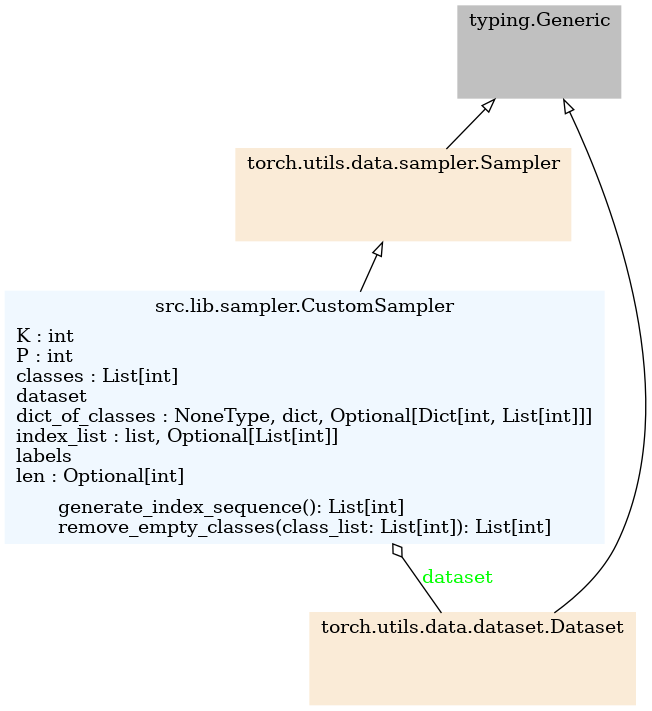
\includegraphics[width=0.6\textwidth]{informatica/pksampler_diagrama_clases}
	\caption{Diagrama de clases de \lstinline{CustomSampler} y sus clases colaboradoras. Este diagrama ha sido creado usando la herramienta \lstinline{pyreverse}, que se ofrece como parte del programa \lstinline{pylint}}
	\label{img:diagrama_clases_CustomSampler}
\end{figure}

En el diagrama de clases \imgref{img:diagrama_clases_CustomSampler} podemos ver que:

\begin{itemize}
	\item \lstinline{CustomSampler} hereda de la clase \lstinline{Sampler} de \lstinline{torch} para introducir el comportamiento deseado a través de un \lstinline{Dataloader} \cite{informatica:pytorch_sampler}.
	      \begin{itemize}
		      \item Un \lstinline{DataLoader} especifica la forma en la que se realiza el \textit{batching} y otros detalles de implementación (por ejemplo, las políticas a seguir para cargar datos cuando trabajamos en paralelo). Uno de sus atributos es el \lstinline{sampler} usado. Escribiendo un \textit{sampler} propio será suficiente para obtener el comportamiento deseado.
		      \item Un \lstinline{Sampler} indica el orden en el que iteramos un \textit{dataset}. Debe implementar el método \lstinline{__len__()}, que muestra el número de datos que ofrecemos, y el método \lstinline{__iter__()}, que indica cómo se itera sobre los índices de los datos almacenados.
	      \end{itemize}
\end{itemize}

En resumen, para realizar \textit{P-K sampling}, especificamos el orden en el que se itera el \textit{dataset} usando la clase \lstinline{CustomSampler}.

Fijados los valores de $P$ y $K$, debemos indicar que el \textit{batch size} sea $P \cdot K$. Esto es claro, pues de otra forma sería imposible generar \textit{batches} en los que haya $P$ individuos representados cada uno con $K$ imágenes.

El funcionamiento de \lstinline{CustomSampler} es el siguiente. Generamos una \textbf{lista de índices} vacía y una lista de imágenes candidatas, que al principio corresponderá al total del \textit{dataset}. Mientras al menos hayan $P$ individuos con al menos $K$ imágenes, realizamos el siguiente proceso:

\begin{enumerate}
	\item Elegimos aleatoriamente $P$ individuos asociados a la lista de imágenes candidatas.
	\item Por cada individuo elegido, seleccionamos $K$ imágenes candidatas suyas aleatoriamente.
	\item Añadimos los índices asociados a las $P \cdot K$ imágenes escogidas al final de la lista de índices y eliminamos dichas imágenes de la lista de candidatas.
\end{enumerate}

Este proceso es realmente sencillo. Sin embargo, realizar optimizaciones para que consuma el menor tiempo posible complica su implementación. Principalmente hemos pre-computado algunos datos, que almacenamos como atributos, para acelerar este proceso:

\begin{itemize}
	\item \lstinline{self.dict_of_classes} es un diccionario en el que cada llave o \textit{key} es el identificador de un individuo (o su clase, en un entorno más amplio que el \textit{AIFR}) y el valor asociado a la llave es una lista de índices de imágenes de ese individuo. Con ello, una vez elegido un individuo al azar, es realmente rápido muestrear $K$ índices de imágenes asociadas.
	\item \lstinline{self.classes} es una lista con los identificadores de individuos que tienen al menos $K$ imágenes, y por tanto, que son candidatos a ser elegidos en un ciclo del proceso anteriormente descrito.
	\item Esto supone que, durante el proceso de generación de índices, debemos mantener en un estado válido estas dos estructuras, lo que añade algo de complejidad a la implementación, aunque supone una mejora en tiempos de ejecución considerable.
\end{itemize}

\begin{observacion}

	Aunque los índices en cada \textit{P-K batch} estén ordenados por individuo, esto no supone un problema al considerar la definición de las funciones de pérdida que estamos usando (véase la \sectionref{isubs:seleccion_de_triples})

\end{observacion}

\section{Aumento de datos} \label{isec:aumentado_datos}

En la \sectionref{isubsubs:observaciones_conclusiones_pksampling} hemos justificado la necesidad de realizar un aumentado de datos en ciertos \textit{datasets}, teniendo mucho cuidado de no saturar la memoria disponible. Por tanto, en el módulo \lstinline{src.lib.data_augmentation} proponemos dos soluciones, que mostramos en el siguiente diagrama de clases:

\begin{figure}[H]
	\centering
	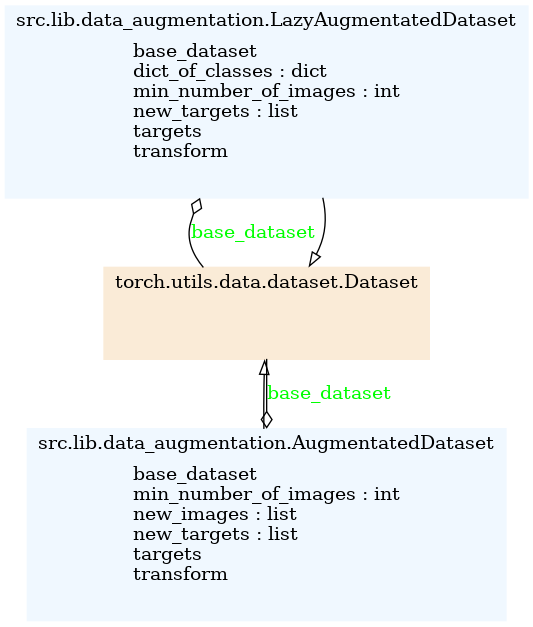
\includegraphics[width=0.6\textwidth]{informatica/diagramas_clases_aumentado_datos}
	\caption{Diagrama de clases de las dos soluciones propuestas para el aumentado de datos. Este diagrama ha sido creado usando la herramienta \lstinline{pyreverse}, que se ofrece como parte del programa \lstinline{pylint}}
	\label{img:diagrama_clases_aumentado_datos}
\end{figure}

En la \imgref{img:diagrama_clases_aumentado_datos} podemos ver que el aumentado de datos se realiza en dos clases que heredan de la clase \lstinline{Dataset} de \lstinline{pytorch}. Gracias a esto, en nuestros \textit{pipelines} trabajamos igualmente con \textit{datasets} aumentados o sin aumentar, sin conocer este detalle. Además, podemos ver que ambas clases exponen la misma interfaz, por lo que podemos intercambiar estas soluciones. Podemos controlar cómo se generan nuevas imágenes gracias al atributo \lstinline{self.transform}.

Para trabajar con el aumentado de datos, indicamos el \textit{dataset} que queremos aumentar, \lstinline{self.base_dataset}, y el número de imágenes mínimo por individuo, \lstinline{self.min_number_of_images}. Dicho valor siempre lo establecemos igual al valor de $K$ que usemos en cada proceso de entrenamiento. Con ello, aseguramos que cada individuo puede participar en al menos un \textit{P-K batch}.

En \lstinline{AugmentedDataset}, localizamos los individuos con menos de \lstinline{self.min_number_of_images} imágenes asociadas. Generamos y almacenamos en memoria no permanente nuevas imágenes para estos individuos, en base a las imágenes que ya tenemos de los individuos. Almacenamos estas imágenes al final del \textit{dataset} (tienen los índices más altos). Pero esto no supone ningún problema gracias a estar usando \textit{P-K sampling}.

En \lstinline{LazyAugmentedDataset} localizamos los individuos con menos de \lstinline{self.min_number_of_images} imágenes asociadas. Generamos nuevos índices para estos individuos, que almacenamos como atributo, sin computar todavía las nuevas imágenes. Cuando queremos acceder a una imagen concreta identificada por un índice, comprobamos si este índice corresponde a una imagen original o una de las imágenes generadas por el aumento de datos. En el primer caso, devolvemos la imagen que ya tenemos almacenada en el conjunto de datos \lstinline{self.base_dataset}. En el segundo caso, generamos la imagen en ese preciso instante y la devolvemos. En ningún momento almacenamos la nueva imagen para su uso posterior. Por tanto, este aumentado de datos apenas supone un aumento en el uso de memoria \textit{RAM} o memoria \textit{GPU}.

El aumento de datos puede llegar a generar muchísimas imágenes nuevas si la distribución de número de imágenes por individuo es mala (como ocurre en \textit{LFW}, véase la \sectionref{isubsubs:imagenes_por_clase_lfw}). Por tanto, el proceso de almacenar las imágenes que hacemos en \lstinline{AugmentedDataset} puede provocar que saturemos la memoria disponible y que el proceso se detenga. Esto motiva el diseño de \lstinline{LazyAugmentedDataset}, que no almacena imágenes en memoria para su posterior uso.

No almacenar las nuevas imágenes en memoria supone el siguiente compromiso:

\begin{itemize}
	\item Si accedemos dos veces al mismo índice, si este se corresponde con una imagen aumentada, no obtendremos la misma imagen.
	\item No se produce un aumento en el consumo de memoria, porque no estamos almacenando ninguna imagen nueva.
	\item El proceso de crear un \textit{dataset} aumentado es más rápido. Pero el acceso a nuevos datos es más lento. En la variante \textit{lazy} tenemos que esperar a que se genere la nueva imagen. Mientras que en la variante normal, ese proceso ya se ha realizado previamente y el acceso es inmediato.
\end{itemize}

Para realizar el aumento de datos estamos utilizando el módulo \lstinline{torchvision.transforms}. En concreto, usamos las siguientes transformaciones:

\begin{itemize}
	\item Un cortado aleatorio de la imagen, usando \lstinline{RandomResizedCrop}. Dicho método toma una porción aleatoria de la imagen, y cambia su tamaño al especificado en la función. El tamaño de las imágenes producidas es igual al tamaño de las imágenes originales.
	\item Una rotación aleatoria, usando \lstinline{RandomRotation}. Rotamos entre 0º y 20º.
	\item Un cambio de contraste aleatorio, usando \lstinline{RandomAutocontrast}.
\end{itemize}

\section{Implementaciones propias de \textit{Datasets}} \label{isec:datasets_customs}

Como ya hemos comentado en la \sectionref{isec:base_datos_usada}, las bases de datos \textit{FG-Net} y \textit{CACD} no se ofrecen como parte de ninguna librería asociada a \lstinline{Pytorch}. Por tanto, tendremos que implementar la descarga, extracción y carga en objetos compatibles con \lstinline{Pytorch}. Estas tareas se realizan en el módulo \lstinline{src.lib.datasets.py}.

Este módulo contiene, además de las dos clases que más adelante estudiamos, las funciones \lstinline{download_fg_dataset} y \lstinline{download_cacd_dataset}, que descargan y extraen los dos \textit{datsets} de internet.

\begin{figure}[H]
	\centering
	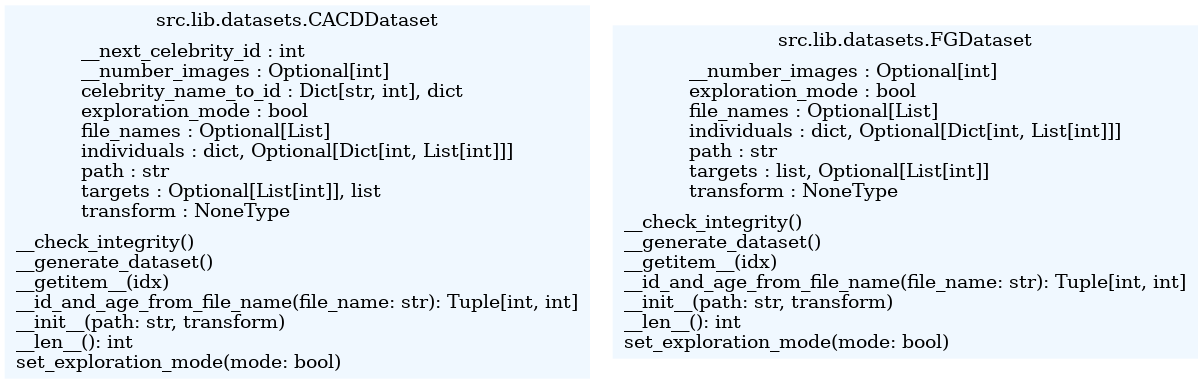
\includegraphics[width=1.0\textwidth]{informatica/diagrama_clases_carga_datos}
	\caption{Diagrama de clases de las implementaciones para los \textit{datasets} \textit{FG-Net} y \textit{CACD}. Este diagrama ha sido creado usando la herramienta \lstinline{pyreverse}, que se ofrece como parte del programa \lstinline{pylint}}
	\label{img:diagrama_clases_datasets}
\end{figure}

En la \imgref{img:diagrama_clases_datasets} podemos ver el diagrama de clases de las dos implementaciones realizadas. Para inicializar estas clases, solo tenemos que especificar la localización del directorio donde se almacenan los datos.

Para poder trabajar correctamente con \lstinline{Pytorch}, debemos especificar el tamaño del \textit{dataset} con el método \lstinline{__len__()} e implementar el acceso a cada elemento del \textit{dataset} con el método \lstinline{__getitem__()}.

A la hora de cargar los datos al \textit{dataset}, realizamos el siguiente proceso:

\begin{itemize}
	\item Tomamos los nombres de todas las imágenes almacenadas en el \textit{dataset}, que guardamos en el atributo \lstinline{self.file_names}.
	\item A partir de los nombres de las imágenes, extraemos el identificador y edad asociados a cada imagen. Para ello usamos el método \lstinline{__id_and_age_from_filename(filename: str)}.
	\item Almacenamos adecuadamente toda esta información para poder devolver dicha información en \lstinline{__getitem__}.
\end{itemize}

El método \lstinline{check_integrity()} comprueba el tamaño del \textit{dataset} para asegurarnos de que no ha habido corrupción de datos en la descarga. El método \lstinline{set_exploration_mode()} permite activar el modo exploración. En dicho modo, \lstinline{__getitem__()} devuelve la imagen con una serie de metadatos asociados almacenados en un diccionario (edad e identidad). En el modo de funcionamiento normal, \lstinline{__getitem__()} devuelve un par con la imagen y la etiqueta de dicha imagen.

\section{Normalización} \label{isubs:normalization_impl}

En la \sectionref{isubs:normalizacion_teoria} hemos justificado por qué es interesante introducir la técnica de normalización en la salida de nuestra red. Además, hemos especificado en qué consiste exactamente esta técnica.

Nuestro objetivo ahora es añadir esta normalización en nuestras redes convolucionales profundas, de forma modular y sencilla. En el módulo \lstinline{src.lib.models}, donde describimos las arquitecturas empleadas a lo largo de toda la experimentación, definimos la clase \lstinline{NormalizedNet}. Dicha clase implementa el patrón de diseño \textit{Decorator} \cite{informatica:design_patterns} \cite{informatica:decorator_pattern}.

En dicho patrón buscamos modificar el comportamiento de un módulo sin cambiar su interfaz. El nuevo comportamiento usa el comportamiento de la clase base, que se adapta de alguna forma. Gracias a no estar modificando la interfaz de la clase base, el resto del código puede trabajar con estos objetos, sin conocer si corresponden a la clase base o a la clase decorada. Esto es justo lo que queremos, porque las funciones que trabajan con nuestra red no deberían depender de la normalización (pensemos por ejemplo en una función que calcula el \textit{Rank@K Accuracy}).

Además, este patrón se basa en la idea de preferir usar composición en vez de herencia (\entrecomillado{composition over inheritance}) \cite{informatica:comp_over_inh}. Mientras que la herencia es estática, la composición es dinámica. Esto, y que el patrón decorador respeta la interfaz de la clase base, permite que podamos combinar varios decoradores a la vez sin problema alguno.

\begin{observacion}

	Este patrón se parece mucho al patrón \textit{Adapter} \cite{informatica:design_patterns} \cite{informatica:adapter_pattern}.

	El objetivo de este patrón es el de adaptar un módulo de código para que implemente una interfaz dada, sin cambiar su comportamiento. Por ejemplo, cuando queremos interactuar con interfaces de terceros usando módulos que no han sido diseñados con dichas interfaces en mente. Por lo tanto, este patrón puede pensarse como el contrario del patrón \textit{Decorator}. Buscamos cambiar la interfaz manteniendo el comportamiento.

\end{observacion}

La clase \lstinline{NormalizedNet} toma una red neuronal como parámetro. Las redes neuronales de \lstinline{pytorch} deben implementar el método \lstinline{forward}, que indica cómo la red computa las salidas a partir de las entradas dadas. Nuestra clase \lstinline{NormalizedNet} implementa este método basándose en el mismo método de la clase base. Usamos el método \lstinline{forward} de la clase base y almacenamos la salida, que normalizamos y devolvemos.

Como ya hemos comentado, el uso de este patrón supone que no estamos cambiando la interfaz de un modelo si lo normalizamos, lo que permite que podamos decidir si queremos trabajar o no con normalización sin que el resto del código tenga que saber este detalle de implementación. Por ejemplo:

\begin{lstlisting}[caption={Ejemplo de uso del patrón \textit{Decorator} para decidir si usamos o no normalización. El resto del código no tiene por qué saber este detalle de implementación, porque no cambiamos la interfaz de la clase}, captionpos=b]
net = LFWResNet18(embedding_dimension = 5)
net = NormalizedNet(net)
\end{lstlisting}

\section{\textit{Hyperparameter Tuning}} \label{isec:hp_tuning}

Como hemos comentado en la \sectionref{isec:hptuning_kfold_cross_validation}, usaremos dos técnicas para realizar el \textit{hyperparameter tuning}: \textit{holdout} y \textit{K-Fold Cross Validation}. Usaremos un código común para los dos enfoques, basado en la librería \textit{optuna}. En función de cuál de los dos enfoques usemos, entrenaremos y evaluaremos de una forma u otra, pero todo el código asociado a la propuesta de nuevas configuraciones e instanciación de las distintas piezas necesarias para llevar a cabo el proceso es el mismo.

Cada \textit{script} que usemos para entrenar y validar definirá una sección de ajuste de hiperparámetros (como comentamos en la \sectionref{isec:pipeline}). Usaremos el \textit{framework} \lstinline{optuna} para realizar una búsqueda en el espacio de hiperparámetros \cite{informatica:optuna_web}. Este \textit{framework} implementa toda la lógica necesaria para proponer valores de hiperparámetros, y en base a los resultados obtenidos gracias a la técnica escogida, proponer nuevos hiperparámetros. Además, usa \lstinline{SQLite} para almacenar los resultados e introducir paralelismo, lo que permite que lancemos varios procesos en los servidores \textit{nGPU}, disminuyendo los tiempos de búsqueda. Como ya hemos comentado, el fichero \lstinline{optuna_queries.sql} contiene las consultas \textit{SQL} para poder acceder a la base de datos donde se almacenan los resultados de la búsqueda.

En la sección de ajuste de hiperparámetros, deberemos configurar \lstinline{optuna} para realizar la búsqueda:

\begin{itemize}
	\item Indicamos qué hiperparámetros queremos explorar, el rango de valores que pueden tomar y sus distribuciones.
	\item Configuramos el proceso que produce el valor numérico a optimizar. En nuestro caso, en función de los hiperparámetros elegidos por \lstinline{optuna}, construimos un modelo u otro, adaptamos la red adecuadamente (por ejemplo, añadiendo o no normalización) y usamos la técnica escogida (\textit{holdout} o \textit{K-Fold Cross validation}) para entrenar y obtener la métrica de error a minimizar.
\end{itemize}

A la hora de aplicar \textit{holdout}, el proceso es muy sencillo. Simplemente separamos el conjunto de entrenamiento en entrenamiento y validación, aprendemos un modelo sobre el conjunto de entrenamiento y evaluamos sobre el conjunto de validación.

Aplicar \textit{K-Fold Cross Validation} no es tan directo, por lo que desarrollamos un módulo \lstinline{src.lib.hyperparameter_tuning}, donde implementamos la función \lstinline{custom_cross_validation}. Dicha función debe generar una métrica a optimizar a partir de una configuración de hiperparámetros dada. La función acepta los siguientes parámetros:

\begin{itemize}
	\item \lstinline{train_dataset}, \textit{dataset} de entrenamiento, sobre el que construiremos los \textit{folds}.
	\item \lstinline{k}, número de \textit{folds} a usar. No confundir con el valor de $K$ en \textit{P-K sampling}.
	\item \lstinline{random_seed}, valor de la semilla aleatoria, para que los resultados sean reproducibles.
	\item \lstinline{network_creator}, función que devuelve una red inicializada aleatoriamente con la arquitectura que queramos trabajar.
	\item \lstinline{network_trainer}, función que toma un \textit{dataloader} y una red neuronal, y ejecuta el entrenamiento devolviendo la red entrenada.
	\item \lstinline{loader_generator}, función que toma un \textit{dataset} que representa uno de los dos bloques (el \textit{fold} de validación o los $k-1$ \textit{folds} de entrenamiento), el tipo de bloque (entrenamiento o validación) y genera un \lstinline{torch.utils.dada.Dataloader} adecuado para poder lanzar el proceso de entrenamiento y el cálculo de la función a optimizar.
	\item \lstinline{loss_function}, función que produce la métrica de error a minimizar.
\end{itemize}

Estamos aplicando el patrón estrategia \cite{informatica:design_patterns} \cite{informatica:strategy_pattern_web}. Pero en vez de estar usando el enfoque clásico en un ambiente de programación orientada a objetos, estamos usando un enfoque funcional. Gracias a esto, podemos usar esta función configurando muy fácilmente qué redes neuronales queremos usar, cómo queremos entrenar la red, cómo queremos trabajar con los datos, ... Y por ende, es muy cómodo trabajar con los hiperparámetros sugeridos por \lstinline{optuna}.

\section{Adaptador para realizar \textit{retrieval}} \label{isubs:impl_retr_adapter}

Como hemos comentado en la \sectionref{isec:triplet_loss}, una de las ventajas de que nuestro modelo aprenda un \textit{embedding} semántico es que podemos adaptar dicho modelo para realizar varias tareas. La tarea que nos interesa en este trabajo es la de \textit{retrieval}.

Esta adaptación se realiza en las clases \lstinline{RetrievalAdapter} y \lstinline{FastRetrievalAdapter}, que se encuentran en el módulo \lstinline{src.lib.models}. Mostramos los diagramas de clase asociados:

\begin{figure}[H]
	\centering
	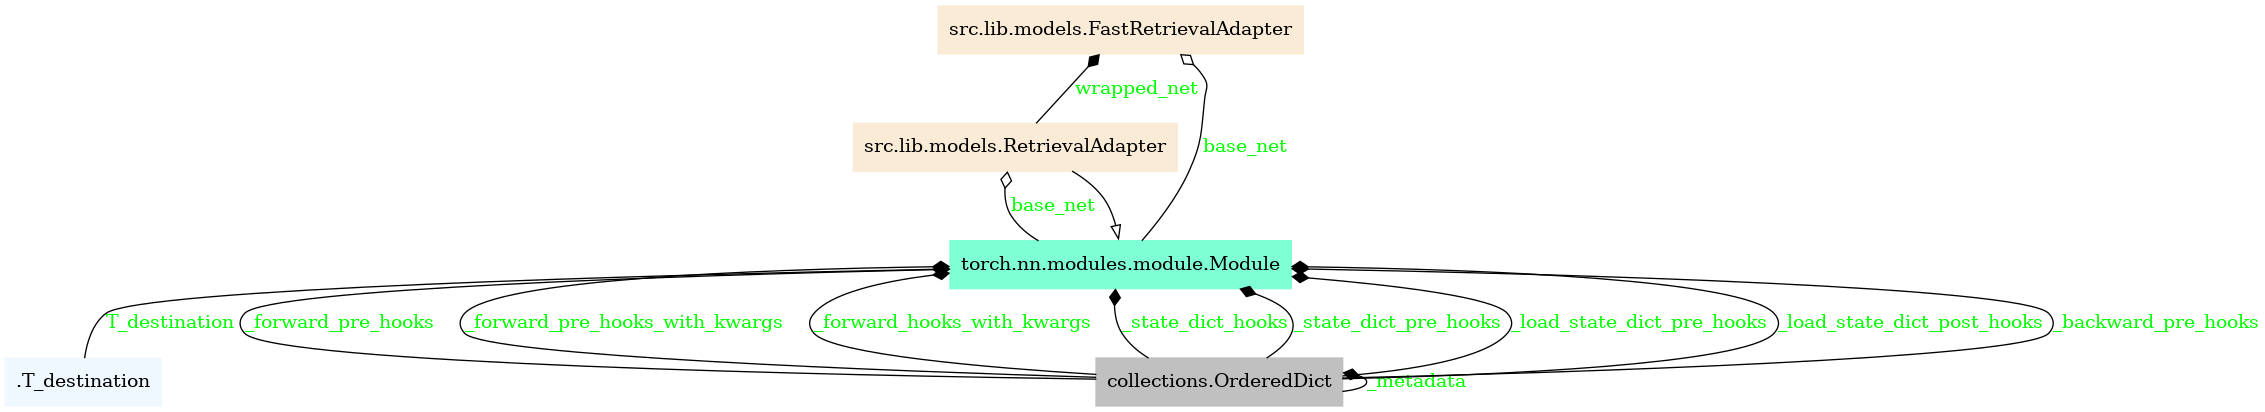
\includegraphics[width=1.0\textwidth]{informatica/diagrama_clases_retrieval}
	\caption{Diagrama de clases de los dos adaptadores. Por el tamaño de \lstinline{torch.nn.Module} solo mostramos los nombres de las clases. Este diagrama ha sido creado usando la herramienta \lstinline{pyreverse}, que se ofrece como parte del programa \lstinline{pylint}}
	\label{img:diagrama_clases_global_adaptadores}
\end{figure}

\begin{figure}[H]
	\centering
	\ajustarsubcaptions
	\begin{subfigure}{.6\textwidth}
		\centering
		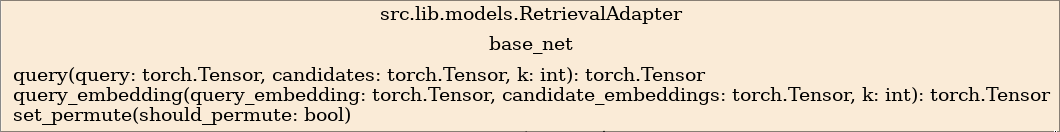
\includegraphics[width=0.9\linewidth]{informatica/diagrama_clases_retrievaladapter}
		\caption{Diagrama de clase de \lstinline{RetrievalAdapter}}
	\end{subfigure}%
	\begin{subfigure}{.4\textwidth}
		\centering
		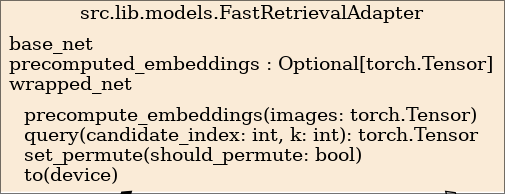
\includegraphics[width=0.9\linewidth]{informatica/diagrama_clases_fastretrieval}
		\caption{Diagrama de clase de \lstinline{FastRetrievalAdapter}}
	\end{subfigure}
	\caption{Diagrama de clase de los dos adaptadores, con toda la información asociada. Estos diagramas han sido creados usando la herramienta \lstinline{pyreverse}, que se ofrece como parte del programa \lstinline{pylint}}
	\label{img:diagramas_clase_concretos_adaptadores}
\end{figure}

En la \imgref{img:diagrama_clases_global_adaptadores} podemos ver que ambas clases implementan la interfaz \lstinline{torch.nn.Module}, que es la interfaz que las redes neuronales y sus componentes deben implementar en \lstinline{pytorch}. Además, \lstinline{RetrievalAdapter} forma parte de \lstinline{FastRetrievalAdapter}. Sin embargo, vamos a introducir una nueva interfaz, por lo que queda claro que ahora sí que vamos a usar el patrón \textit{Adapter} (en el \sectionref{isubs:normalization_impl} hablamos de los patrones \textit{Adapter} y \textit{Decorator} en profundidad).

En la \imgref{img:diagramas_clase_concretos_adaptadores} podemos ver que no estamos buscando trabajar con la interfaz de \lstinline{torch.nn.Module}, sino que buscamos trabajar con una nueva interfaz, asociada a la tarea de \lstinline{retrieval} (véase la \sectionref{ich:descrp_problema}). Para ello, la clase \lstinline{RetrievalAdapter} define dos métodos relevantes, que son los que introducen una nueva interfaz:

\begin{itemize}
	\item \lstinline{query} toma una imagen \textit{key}, una lista de imágenes que forman la base de datos y el número de imágenes $k$ que queremos que devuelva la consulta. Devuelve los índices asociados a las mejores $k$ imágenes de la base de datos.
	      \begin{itemize}
		      \item Tenemos imágenes como entradas, así que debemos almacenar la red neuronal que computa los \textit{embeddings} para transformar estas imágenes.
		      \item Esto lo hacemos con el atributo \lstinline{self.base_net}.
	      \end{itemize}
	\item \lstinline{query_embedding} realiza la misma tarea, pero en vez de pasar la imagen \textit{key} y las imágenes que forman la base de datos, pasamos directamente los \textit{embeddings} de estas imágenes. En este caso:
	      \begin{itemize}
		      \item Tenemos que tener cuidado de usar la misma red neuronal que la que tenemos almacenada en \lstinline{self.base_net}, para evitar errores lógicos.
		      \item \lstinline{src.base_net} no participa en el cómputo de este método.
	      \end{itemize}
	\item \lstinline{set_permute} trata sobre detalles sobre como trabajamos la representación de los tensores de \textit{batches} en memoria.
\end{itemize}

La clase \lstinline{FastRetrievalAdapter} añade algunas modificaciones para acelerar los tiempos de cómputo:

\begin{itemize}
	\item Podemos ver en la \imgref{img:diagramas_clase_concretos_adaptadores} que esta clase se compone de un modelo que computa el \textit{embedding} semántico, \lstinline{self.base_net}, y un modelo que ya está adaptado a la tarea de \textit{retrieval}, \lstinline{self.wrapped_net}. \lstinline{self.wrapped_net} es el resultado de construir un objeto de la clase \lstinline{RetrievalAdapter} usando \lstinline{self.base_net}.
	\item En la \sectionref{isubs:rank_at_k} se especifica de qué forma se va a usar la adaptación. Siempre tomaremos una base de datos de imágenes, extraeremos una imagen que usaremos como \textit{key}, y realizaremos la \textit{query} contra el resto de imágenes de la base de datos.
	\item Por tanto, en el método \lstinline{precompute_embeddings} pasamos toda la base de datos de imágenes, calculamos su proyección en el \textit{embedding} usando \lstinline{self.base_net}, y almacenaremos estos datos.
	\item Con esto, el método \lstinline{query} simplemente especifica el índice de la \textit{key} y el número $k$ de individuos más parecidos que queremos seleccionar. Y usando \lstinline{self.wrapped_net} con su método \lstinline{query_embedding}, realizamos el cómputo sobre los \textit{embeddings} precomputados.
\end{itemize}

\begin{sloppypar}
	\lstinline{FastRetrievalAdapter} claramente está utilizando el patrón \textit{Decorator} (del que ya hemos hablado en la \sectionref{isubs:normalization_impl}) sobre la clase \lstinline{RetrievalAdapter}. Para acelerar los tiempos de ejecución, simplemente realizamos un pre-cómputo y utilizamos la implementación de la clase \lstinline{RetrievalAdapter}.
\end{sloppypar}

\section{Separación de datos imponiendo clases disjuntas}

A la hora de separar el \textit{dataset} completo en subconjuntos (entrenamiento, validación y \textit{test}), la opción más utilizada es la de usar muestreo aleatorio para seleccionar qué elementos van a un conjunto u otro. En el problema que estamos resolviendo esto puede no ser adecuado por las siguientes peculiaridades:

\begin{itemize}
	\item Un individuo con al menos $K$ imágenes asociadas puede acabar teniendo menos de $K$ imágenes asociadas en el subconjunto de entrenamiento. Esto provoca que no pueda participar en ningún \textit{P-K batch} en el proceso de aprendizaje.
	\item Además, podemos acabar con conjuntos de validación y \textit{test} en los que muchos individuos han sido vistos durante el proceso de entrenamiento. En la aplicación real del modelo vamos a encontrarnos con muchas identidades nunca vistas (potencialmente siempre será así).
\end{itemize}

Por tanto, es conveniente que usemos una separación de datos en la que las identidades (clases, en un ambiente más amplio que el \textit{AIFR}) sean disjuntas. Esto es, que no existan individuos con imágenes asociadas en más de un conjunto de datos.

Las dos técnicas de separación (clásica e identidades disjuntas) se implementan en el módulo \lstinline{src.lib.split_dataset}, en las funciones \lstinline{split_dataset} y \lstinline{split_dataset_disjoint_classes}

\section{Logging de métricas} \label{isec:loggin_metricas}

\begin{figure}[H]
	\centering
	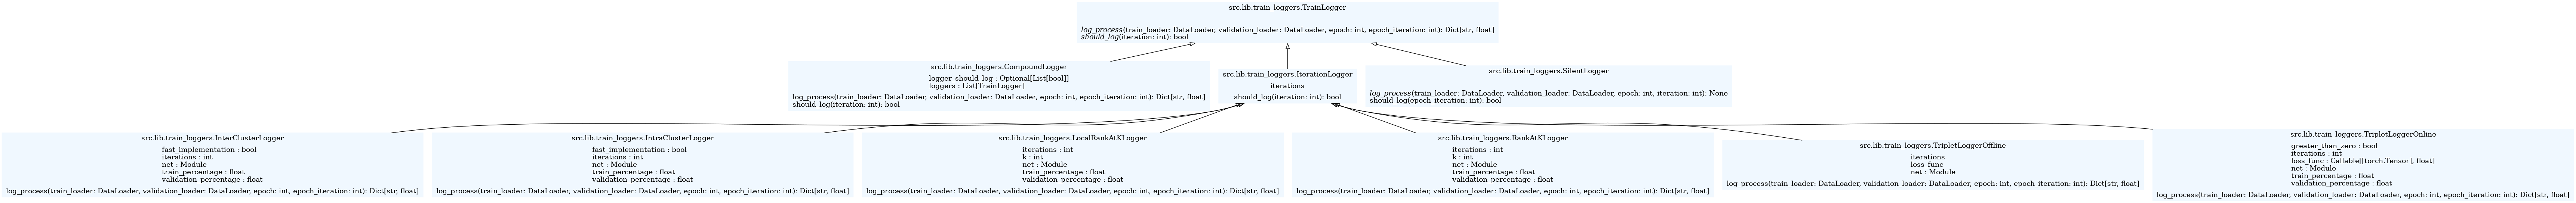
\includegraphics[width=1.0\textwidth,height=\textheight,keepaspectratio]{informatica/diagrama_loggers}
	\caption{Diagrama de clases del módulo \lstinline{src.lib.train_loggers}. Este diagrama ha sido creado usando la herramienta \lstinline{pyreverse}, que se ofrece como parte del programa \lstinline{pylint}}
	\label{img:diagrama_clases_loggers}
\end{figure}
% TODO -- Arreglar esta imagen, no se ve nada

El módulo \lstinline{src.lib.train_loggers} se encarga de introducir el cálculo y visualización de métricas en el proceso de entrenamiento de forma cómoda, modular y extensible. Nuestro objetivo es definir el proceso de \textit{logging} de forma externa al bucle de entrenamiento. Así podremos cambiar las métricas observadas sin tener que modificar el código que implementa el bucle de entrenamiento.

En la \imgref{img:diagrama_clases_loggers} podemos ver la siguiente estructura:

\begin{itemize}
	\item La clase abstracta \lstinline{Trainlogger} define la interfaz que queremos que todos los \textit{loggers} implementen. Dicha interfaz se compone de dos métodos:
	      \begin{itemize}
		      \item \lstinline{log_process} que muestra los valores de ciertas métricas tomando como entradas los datos de entrenamiento, los datos de validación, la época en la que nos encontramos en el proceso de entrenamiento y la iteración dentro de dicha épica.
		      \item \lstinline{should_log} que decide si debemos mostrar o no las métricas para una iteración global del proceso de entrenamiento.
	      \end{itemize}
	\item Gracias a esta interfaz, el bucle de entrenamiento puede mostrar métricas solo cuando \lstinline{should_log} lo indique, pasando todos los datos necesarios a \lstinline{log_process}.
	\item La clase \lstinline{SilentLogger} ofrece una implementación trivial de la interfaz. \lstinline{should_log} siempre devuelve falso y \lstinline{log_process} no realiza ninguna acción.
	\item El resto de clases tienen la misma lógica para decidir cuándo mostrar las métricas. Por tanto, la clase abstracta \lstinline{IterationLogger} implementa dicha lógica compartida, dejando todavía como método abstracto a \lstinline{log_process}.
	\item Los \textit{loggers} que vemos en la parte baja del diagrama son \textit{loggers} concretos que implementan cada uno \lstinline{log_process} con el cálculo y visualización de métricas concretas.
	\item La clase \lstinline{CompoundLogger} implementa el \textbf{patrón de diseño \textit{composite}}.
\end{itemize}

Como acabamos de comentar, la clase \lstinline{CompoundLogger} implementa el patrón de diseño \textit{composite} \cite{informatica:design_patterns}. En dicho patrón buscamos definir la lógica de ciertos componentes en función del agregado de otros componentes. En nuestro caso, buscamos definir un objeto que implemente la interfaz \lstinline{TrainLogger} combinando varios \textit{loggers} en uno solo. Para ello, guardamos una lista de objetos de tipo \lstinline{TrainLogger}. La función \lstinline{should_log} consulta a todos los objetos guardados si quieren mostrar métricas, haciendo uso de la misma función \lstinline{should_log}. En cuyo caso, se llama a los correspondientes métodos \lstinline{log_process}. Gracias a esto, en un \textit{script} de \lstinline{Python} podemos configurar nuestro \textit{logging} con el siguiente código:

\begin{lstlisting}[language=python, caption=Ejemplo de configuración del \textit{logging} de un entrenamiento con nuestro sistema propio. Se ve claramente la ventaja de usar un patrón \textit{composite} a la hora de configurar qué \textit{loggers} queremos usar, captionpos=b]

# Define the loggers we want to use
triplet_loss_logger = TripletLoggerOnline(... params ... )
cluster_sizes_logger = IntraClusterLogger(... params ... )
intercluster_metrics_logger = InterClusterLogger( ... params ... )
rank_at_one_logger = RankAtKLogger( ... params ... )
rank_at_k_logger = RankAtKLogger( ... params ... )
local_rank_at_one_logger = LocalRankAtKLogger( ... params ... )
local_rank_at_k_logger = LocalRankAtKLogger( ... params ... )

# Combine them in a single logger
logger = CompoundLogger([
    triplet_loss_logger,
    cluster_sizes_logger,
    intercluster_metrics_logger,
    rank_at_one_logger,
    rank_at_k_logger,
    local_rank_at_one_logger,
    local_rank_at_k_logger,
])
\end{lstlisting}

Hemos usado \textbf{dos técnicas para mostrar las métricas calculadas}. La primera y más sencilla ha sido \textbf{imprimir por pantalla} los valores obtenidos. Esta técnica no es suficiente porque no podemos guardar de forma estructurada los históricos de entrenamientos, ni facilita estudiar de forma visual el comportamiento del entrenamiento. Por tanto, hemos usado como segunda técnica el servicio \textbf{\textit{Weights and Biases} o \textit{WANDB}} \cite{informatica:wandb_web}. Este servicio permite registrar métricas de forma muy sencilla, relegando a dicho servicio:

\begin{itemize}
	\item El control de históricos de entrenamiento.
	\item La visualización de los procesos de entrenamiento.
	\item El registro de parámetros globales usados en cada entrenamiento.
\end{itemize}

Para registrar todos los parámetros globales, creamos un diccionario de \lstinline{Python} en el que definimos los valores de dichos parámetros. Este diccionario, al que llamamos \lstinline{GLOBALS}, se registra directamente en la plataforma \textit{WANDB}. Los parámetros globales definen hiperparámetros del proceso de entrenamiento (por ejemplo, los valores de $\{P, K\}$), directorios en los que guardamos archivos, qué entorno de ejecución estamos usando o si queremos saltar ciertas secciones del \textit{pipeline} (véase la \sectionref{isec:pipeline}).
